\section{Evaluation}
\label{sec:eval}

\subsection{Experimental Setup}

\subsubsection{Hardware}

We ran our tests on a mid-2012 MacBook Pro with a 2.6 GHz Core i7 processor,
8GB RAM, and an NVIDIA GeForce GT 650M graphics card with 1GB memory.


\subsubsection{The Router}

We implemented a software router framework capable of running in two modes:
CPU-only or CPU/GPU. We use the router in CPU-only mode to gather a baseline
against which we can compare the performance of CPU/GPU mode. In either mode,
the framework handles gathering batches of packets, passing them to a
``pluggable'' packet processing function, and forwarding them based on the
results of processing. 

We implemented three processing functions: one that does longest prefix match,
one that does firewall rule matching, and one that does both. For each we
implemented CPU version and a GPU version (the GPU version is a CUDA kernel
function). \TODO{Mention that the CPU-only versions only use one core?}

\subsubsection{Packet Generation}
\TODO{Matt: describe using click generator for ``full-on'' tests and packet trace for ``real-world'' tests}

\subsubsection{Packet Processing}
\label{sec:eval-proc}

\noindent \textbf{Longest Prefix Match.} Describe the FIB we use...\\
\TODO{Bruno: describe using RouteViews? FIB...}

\noindent \textbf{Firewall Rule Matching.} To evaluate the performance of our
router's firewall rule matching function, we generate a set of random firewall
rules. The 5-tuple values for our random rules are chosen according to the
distributions in \cite{Rovniagin}. For example, we use the probabilities in
Table~\ref{tab:proto-dist}, taken from \cite{Rovniagin}, to pick a new rule's
protocol. Similar statistics were used to pick source/destination address/port.

\begin{table}[htbp]
   \centering
   \begin{tabular}{ l l } 
      \toprule
      \textbf{Protocol}  & \textbf{Prevelance in Rules} \\
      \midrule
	  TCP & 75\% \\
      UDP & 14\% \\
	  ICMP & 4\% \\
	  * & 6\% \\
	  Other & 1\% \\
      \bottomrule
   \end{tabular}
   \caption{Protocol distribution in firewall rules}
   \label{tab:proto-dist}
\end{table}

\subsection{Evaluation Metrics}
\label{sec:metrics}

We use three different metrics to evalute our router's performance. The results
presented in \S\ref{sec:results} present these values averaged over 30 seconds
of router operation.

\medskip \noindent \textbf{Bandwidth.} No router performance evaluation would
be complete without considering bandwidth, and so we measure the number of 64
byte packets forwarded by our router per second, from which we calculate
bandwidth in gigabits per second. For comparison, the norm for core routers is
about 40 Gbps with high-end routers currently maxing out around 100 Gbps.

\medskip \noindent \textbf{Latency.} Bandwidth only tells part of the story,
however; the delay a single packet experiences at a router is important as well
(for some applications, it is more important than bandwidth). Since some
optimizations aimed at increasing our router's bandwidth increase latency as
well (such as increasing batch sizes), measuring latency is important.

We measure both the minimum and maximum latencies of our router. The maximum
latency is the time from the arrivial of the first packet of a batch to the
time it is forwarded; the minimum latency is the same but for the last packet
of a batch.

\medskip \noindent \textbf{Processing Time.} We also consider a microbenchmark:
the time spent in the packet processing function itself (i.e., doing the longest
prefix match lookup or matching against firewall rules). This is largely a
sanity check; we expect to see the GPU perform much better here, though actual
performance (measured by bandwidth and latency) depends on many other factors
(like the time spent copying data to/from the GPU).


\subsection{Results}
\label{sec:results}

Our router went through four iterations, each one an optimization based on what
we learned from the results of the last. We therefore present our results in
four stages, guiding the reader through our design process.

\subsubsection{Iteration One}

We began by na\"{i}vely implementing the design presented in
\S\ref{sec:system-design}; at this point, we made no optimizations --- the goal
was building a functioning GPU-based router.

Not surprisingly, it performed underwhelmingly. The GPU version of our router
achieved roughly 80\% of the bandwidth the CPU version did
(Figure~\ref{fig:iter1-bw}) and also had (max and min) latencies 1.3X longer
(Figure~\ref{fig:iter2-lat}). The processing time is not to blame; as expected,
the GPU performs the actual packet processing much faster than the CPU
(Figure~\ref{fig:iter1-proc}). A quick examination of the time spent performing
different functions (Figure~\ref{fig:iter1-gpu-breakdown}) explains where the
GPU router is losing ground: although it spends less time processing, it has to
copy packets to the GPU for processing and copy the results back, tasks the CPU
version doesn't need to worry about (Figure~\ref{fig:iter1-cpu-breakdown}).

\begin{figure}
    \centering
    \subfigure[Bandwidth vs. Batch Size]{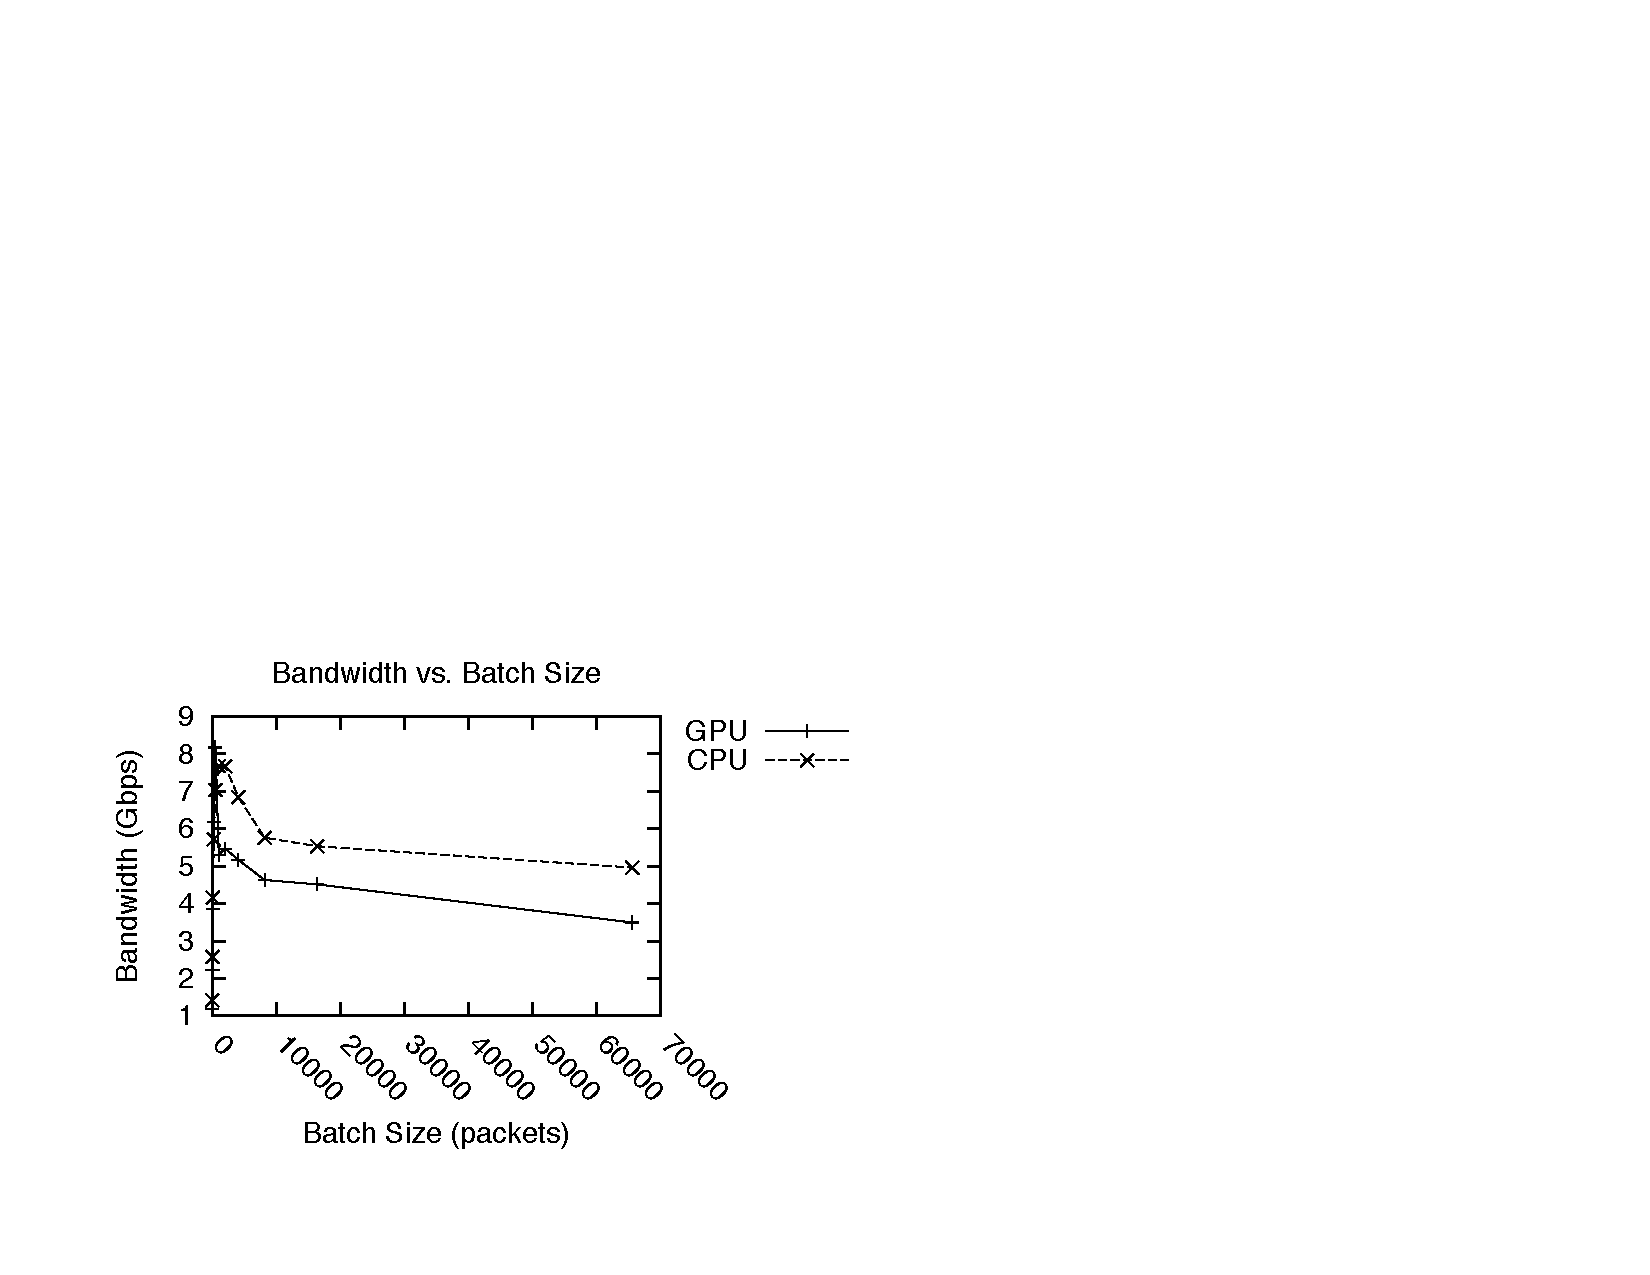
\includegraphics[height=3.5cm]{figs/batch_size_both_par_bw.pdf}\label{fig:iter1-bw}}
	\medskip

    \subfigure[Latency vs. Batch Size]{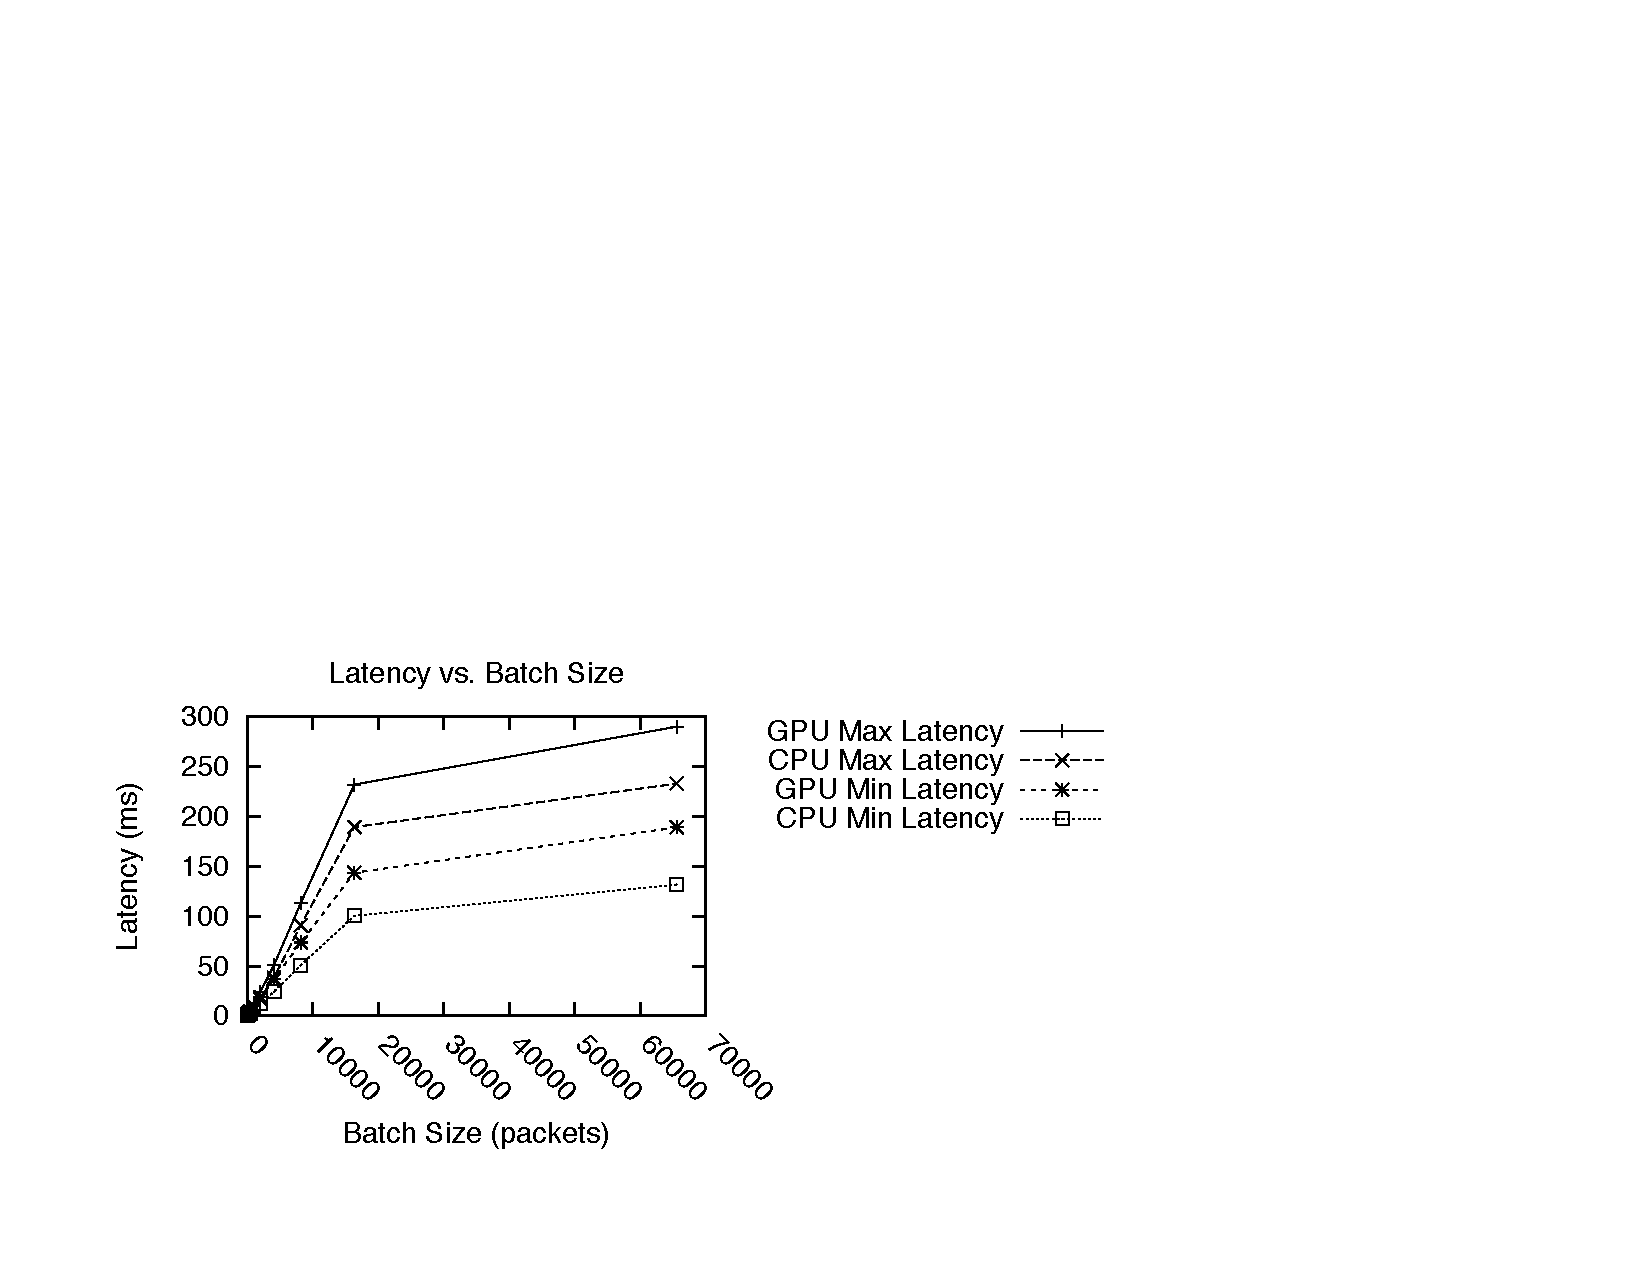
\includegraphics[height=3.5cm]{figs/batch_size_both_par_lat.pdf}\label{fig:iter1-lat}}

	\medskip
    
	\subfigure[Processing Time vs. Batch Size]{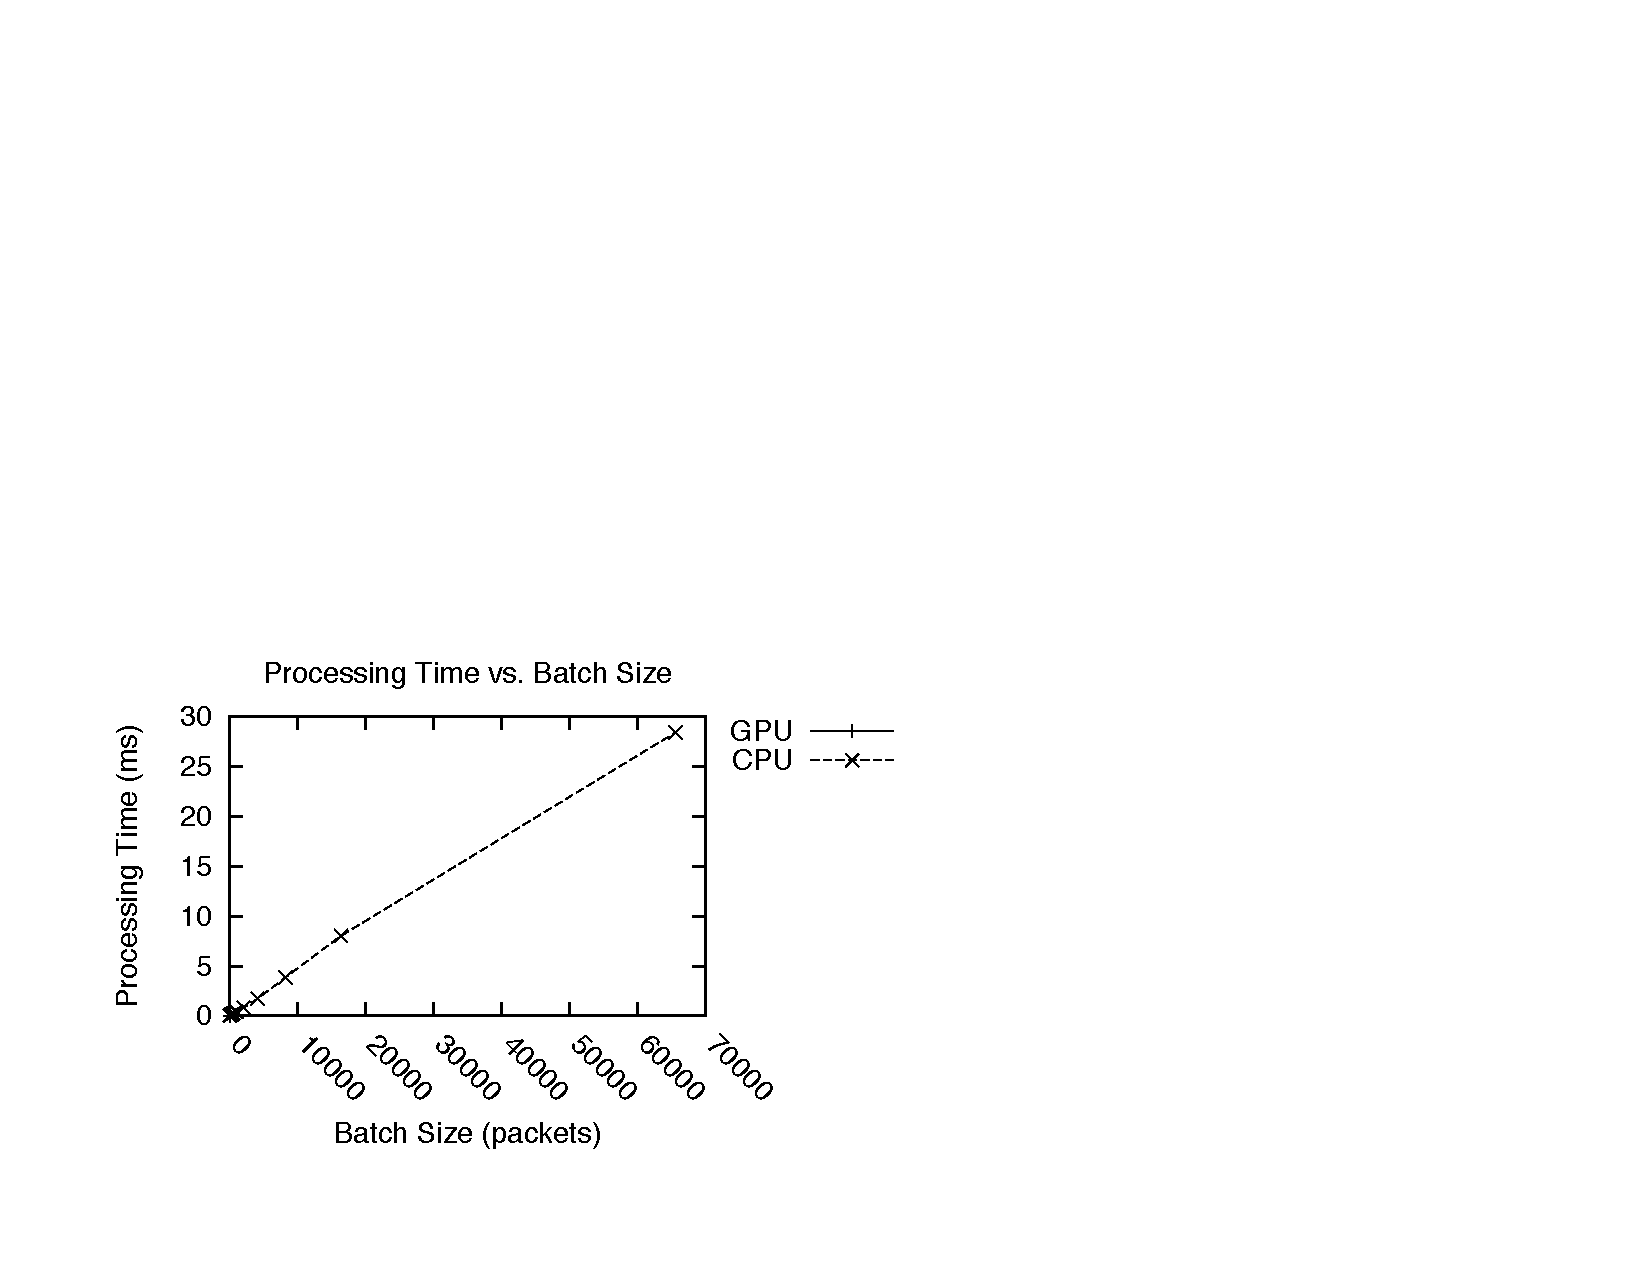
\includegraphics[height=3.5cm]{figs/batch_size_both_par_proc.pdf}\label{fig:iter1-proc}}
	\medskip
	
	\subfigure[Breakdown of GPU Time]{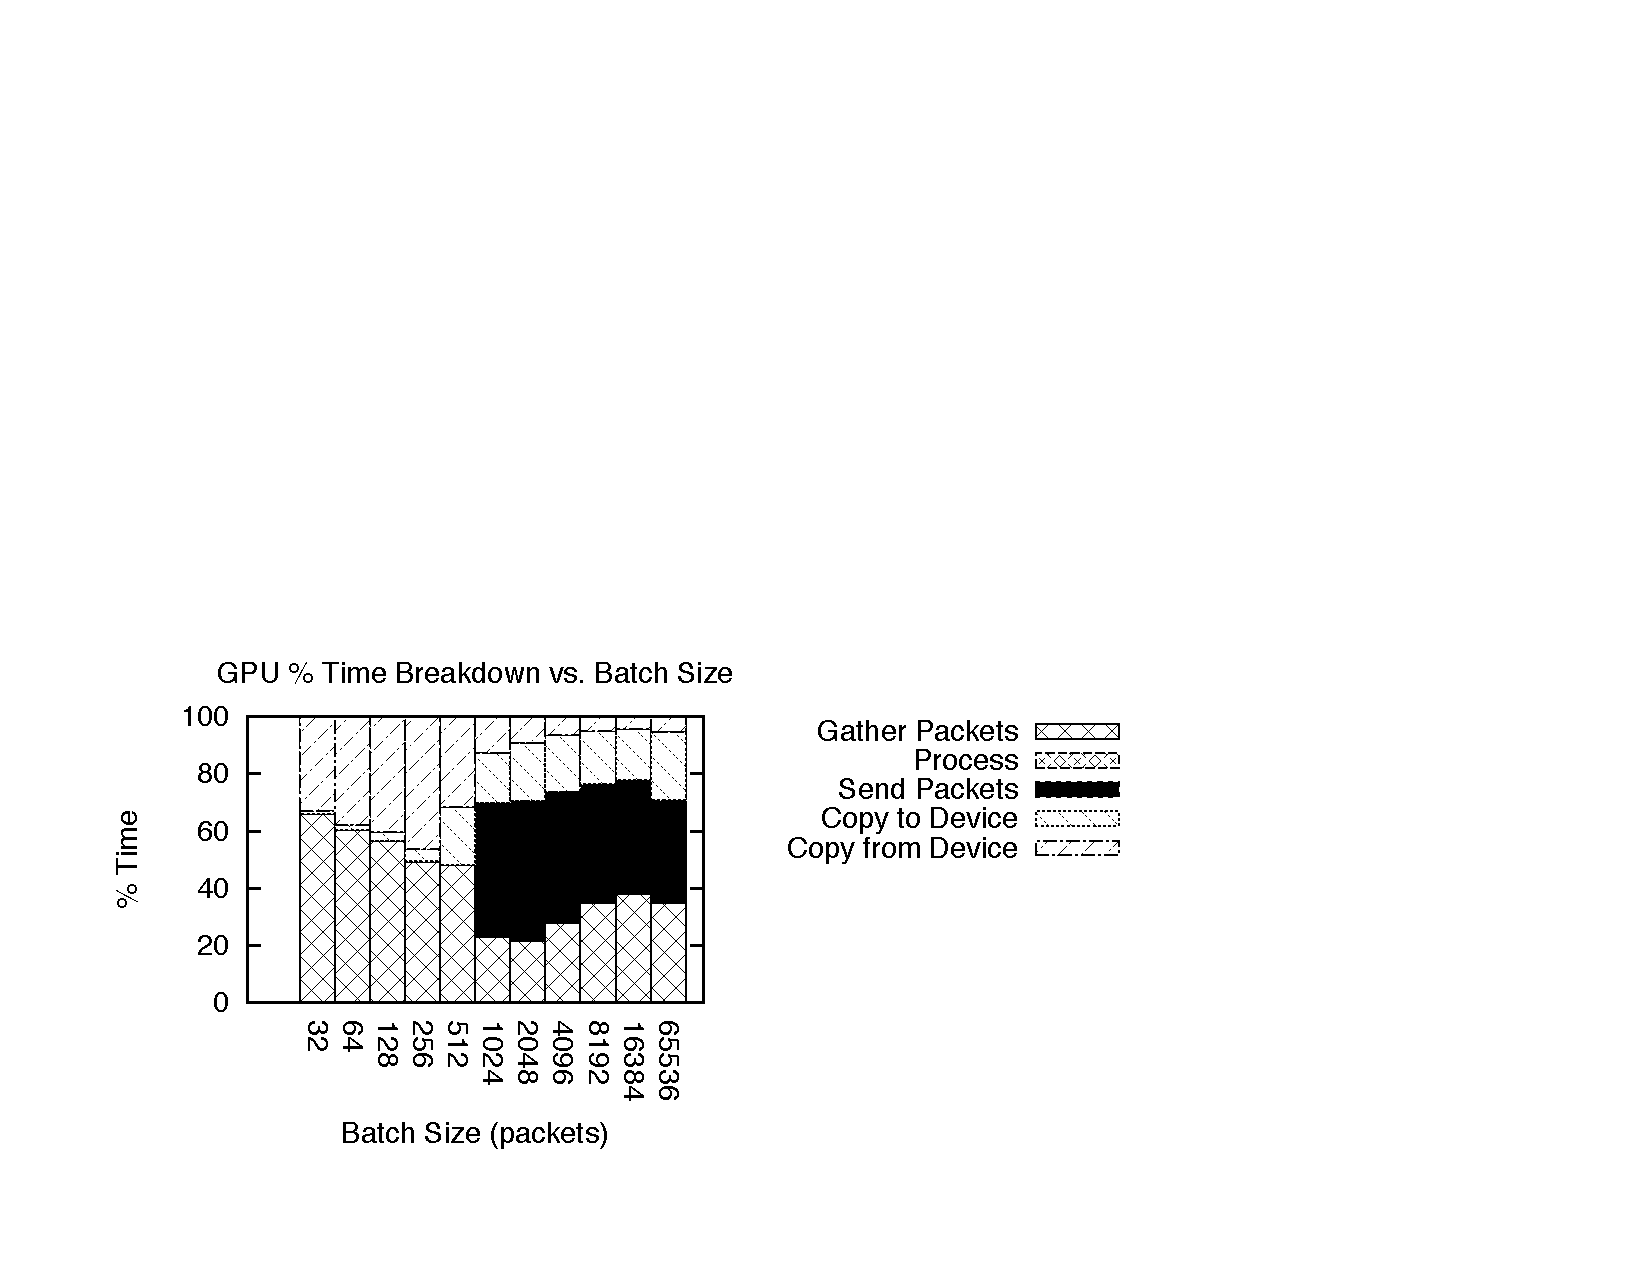
\includegraphics[height=3.5cm]{figs/batch_size_both_par_gpu_p.pdf}\label{fig:iter1-gpu-breakdown}}
	
	\medskip
	\subfigure[Breakdown of CPU Time]{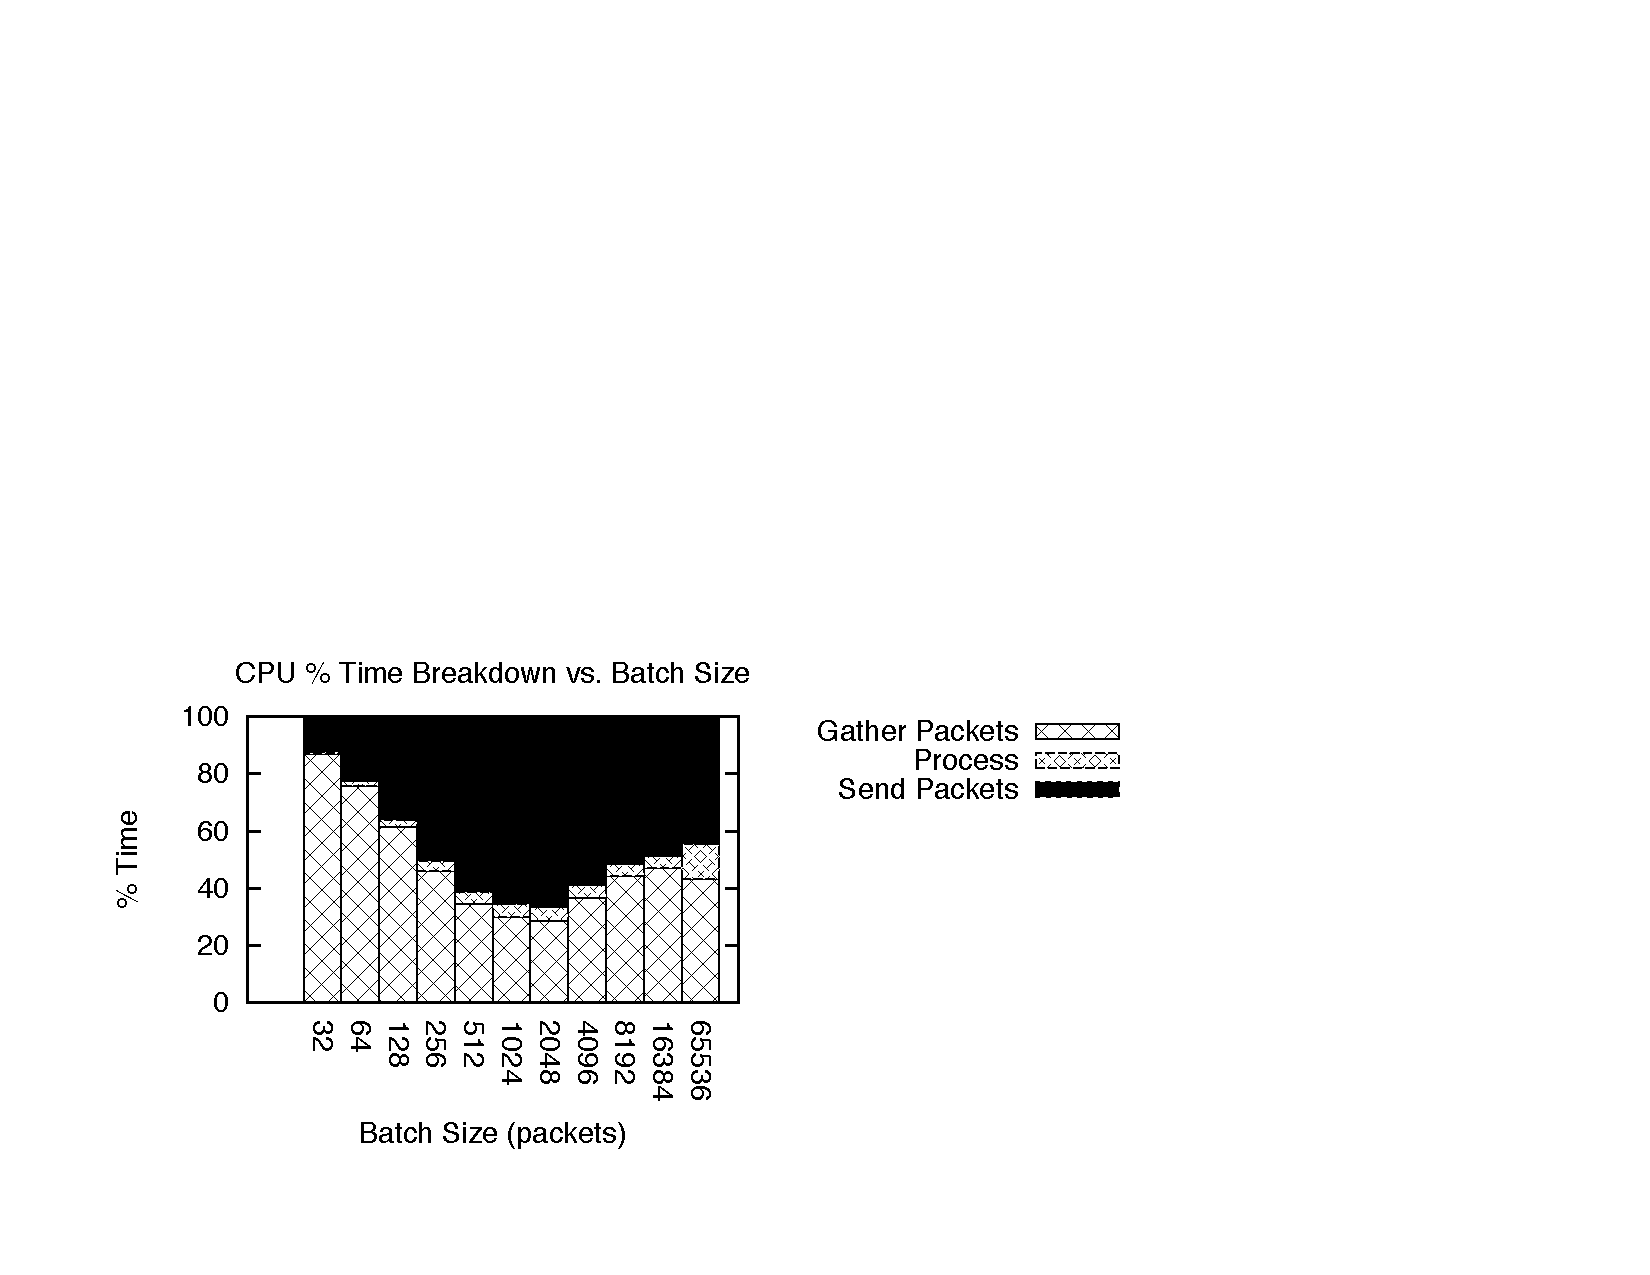
\includegraphics[height=3.5cm]{figs/batch_size_both_par_cpu_p.pdf}\label{fig:iter1-cpu-breakdown}}

    \caption{Iteration 1 Results}
	\label{fig:iter1}
\end{figure}


\subsubsection{Iteration Two}

Since both of our packet processing functions operate only on the data carried
by the packet header, we can reduce the time spent copying data to the GPU by
copying only the packet headers. Unfortunately, the results do not contain
unnecessary information, and cannot easily be condensed (this is not completely
true --- it is probably possible to compress the results, though we do not
explore this here).

Figure~\ref{fig:iter2} shows the performance of the second iteration of our
router. Reducing the number of bytes copied to the GPU has closed the gap
between the CPU-only and the CPU/GPU routers in terms of bandwidth and latency,
but the CPU/GPU router still doesn't perform any better. Even though we have
all but eliminated copy time to GPU, Figure~\ref{fig:iter2-gpu-breakdown}
suggests that we should try to cut down copy time from the GPU as well.

\begin{figure}
    \centering
    \subfigure[Bandwidth vs. Batch Size]{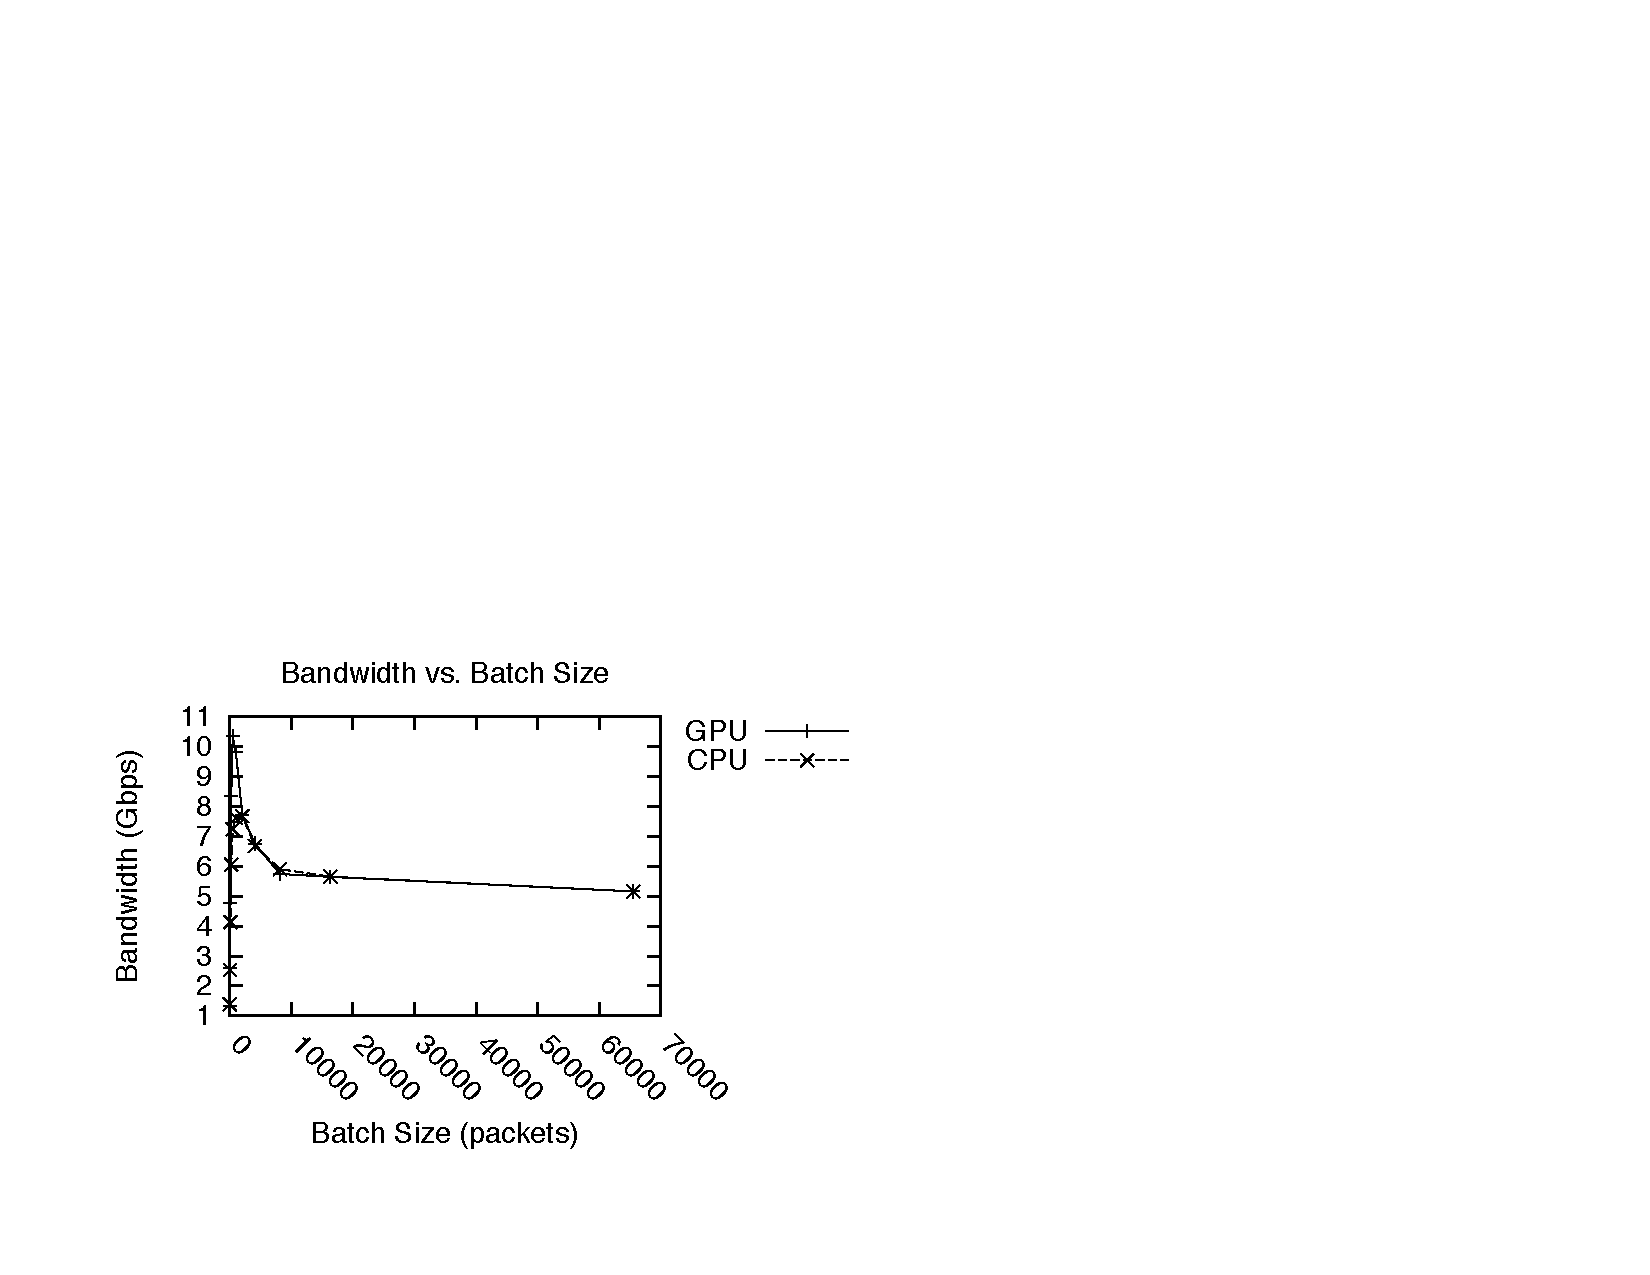
\includegraphics[height=4cm]{figs/batch_size_header_both_par_bw.pdf}\label{fig:iter2-bw}}

	\medskip
    \subfigure[Latency vs. Batch Size]{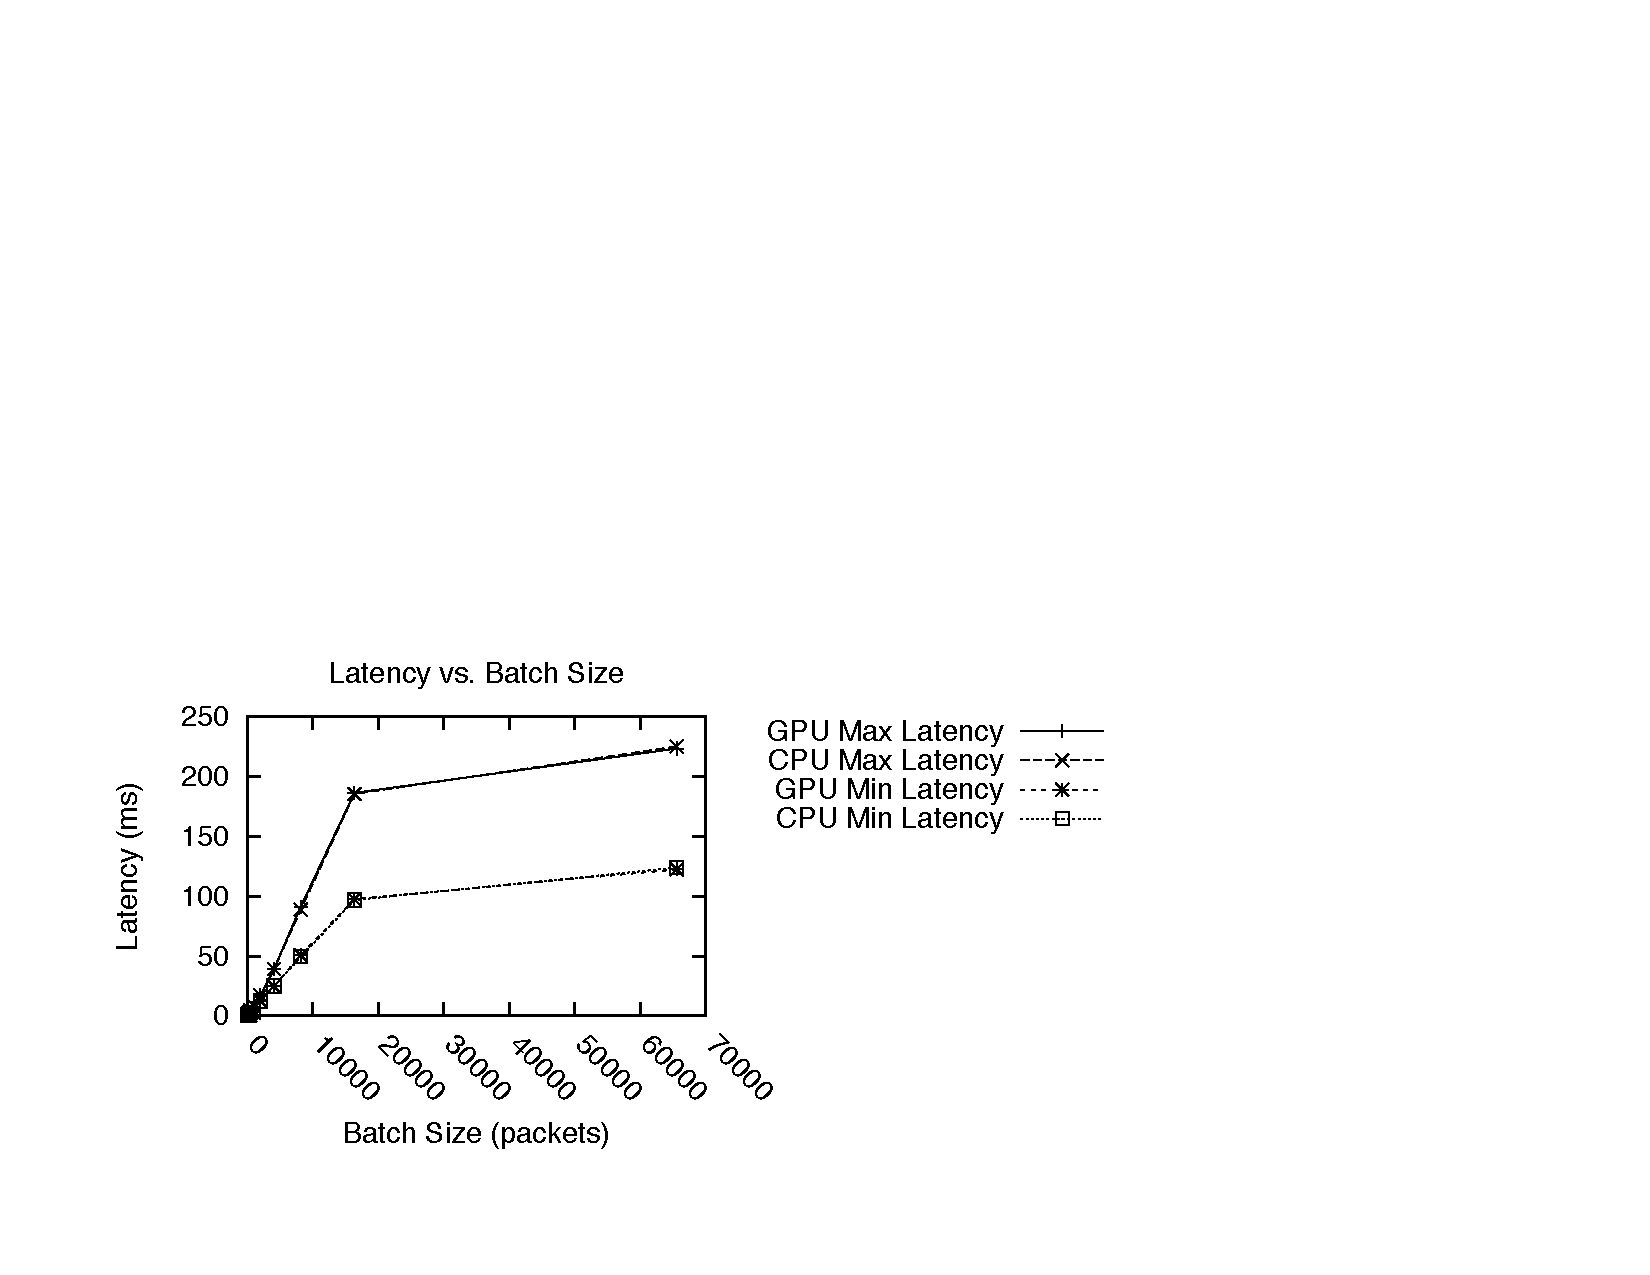
\includegraphics[height=4cm]{figs/batch_size_header_both_par_lat.pdf}\label{fig:iter2-lat}}

   	\medskip
	\subfigure[Breakdown of GPU Time]{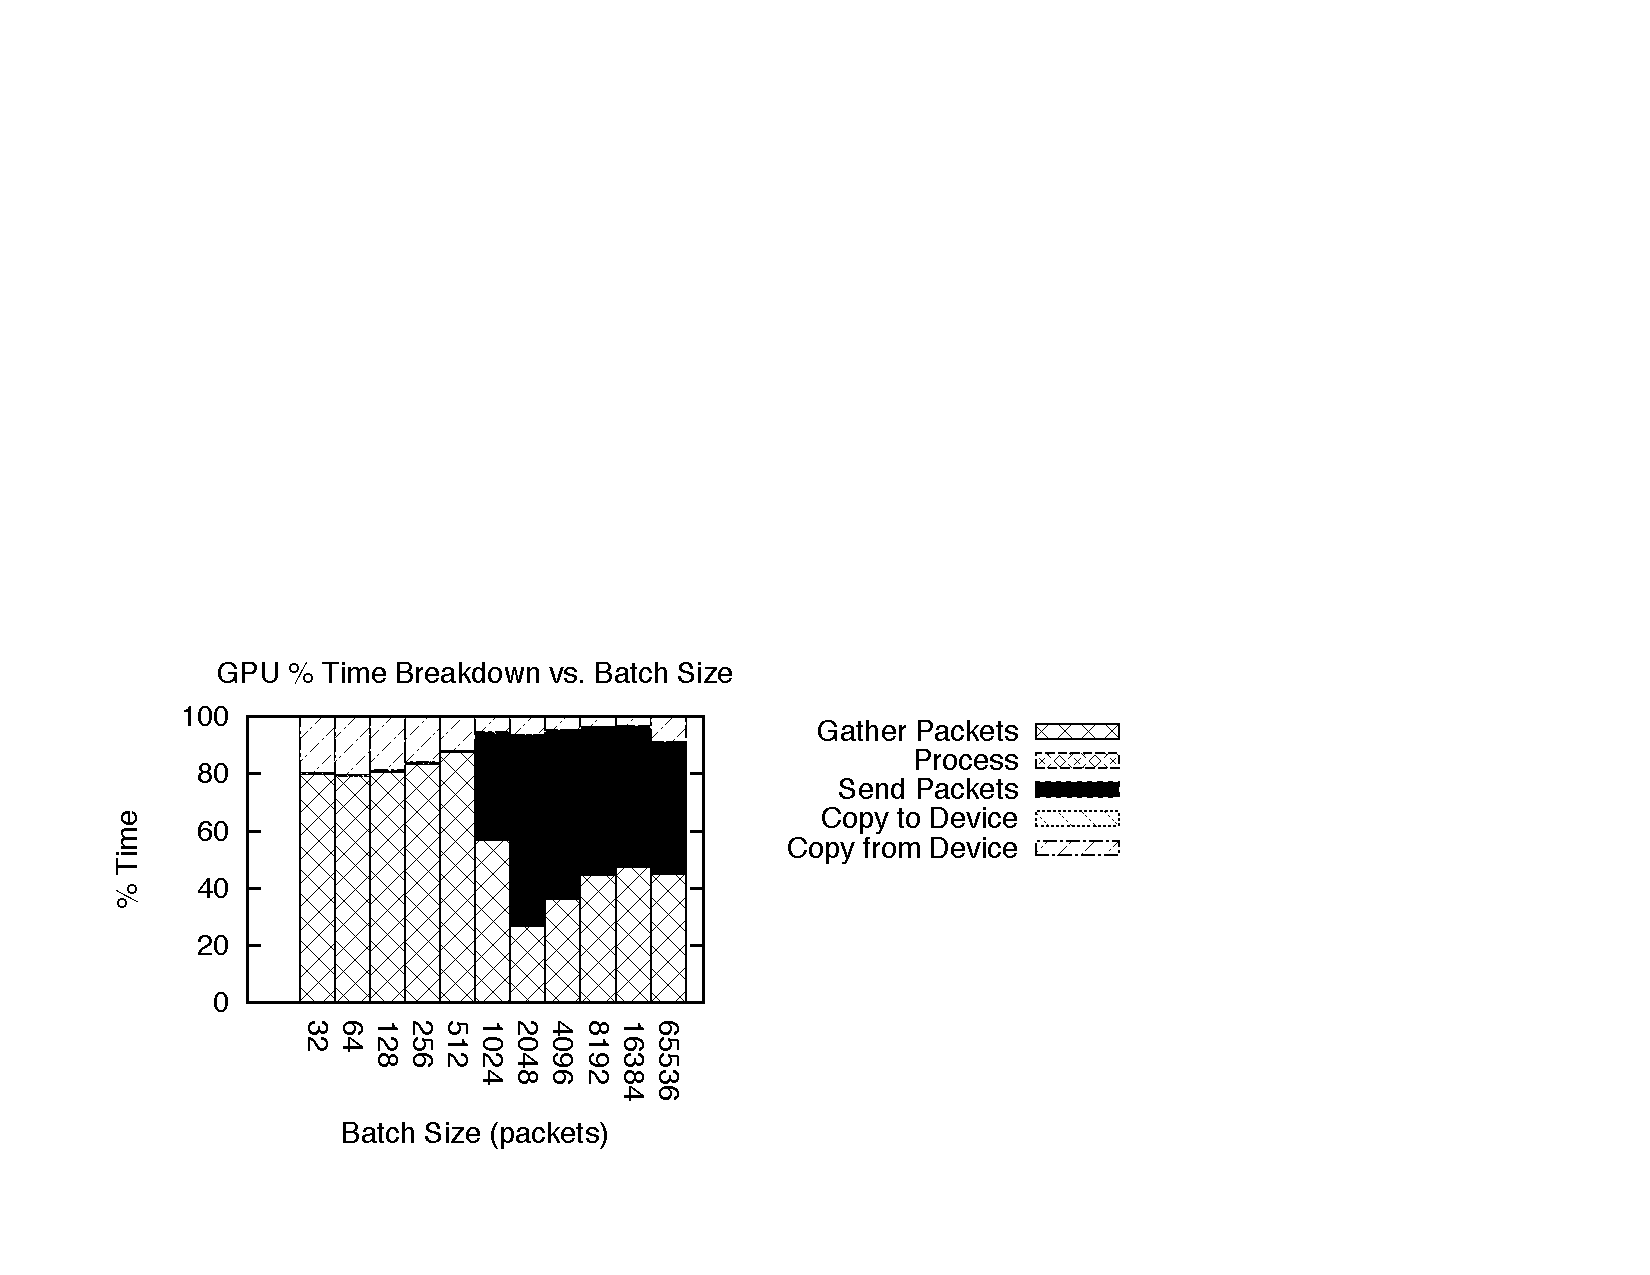
\includegraphics[height=4cm]{figs/batch_size_header_both_par_gpu_p.pdf}\label{fig:iter2-gpu-breakdown}}

    \caption{Iteration 2 Results}
	\label{fig:iter2}
\end{figure}


\subsubsection{Iteration Three}

Unfortunately, there is no unnecessary data being copied back from the GPU as
there was being copied to it; we must find another way to reduce the
copy-from-GPU overhead. Instead, we modify our router's workflow to take
advantage of mapped memory (\S\ref{sec:gpu-issues}).

This gives the CPU/GPU router a tiny edge over the CPU-only router
(Figure~\ref{fig:iter3}), but the gains are small (as Amdahl's Law would
suggest --- the copy-from-device time we eliminated was a small portion of the
total time in Figure~\ref{fig:iter2-gpu-breakdown}).


\begin{figure}
    \centering
    \subfigure[Bandwidth vs. Batch Size]{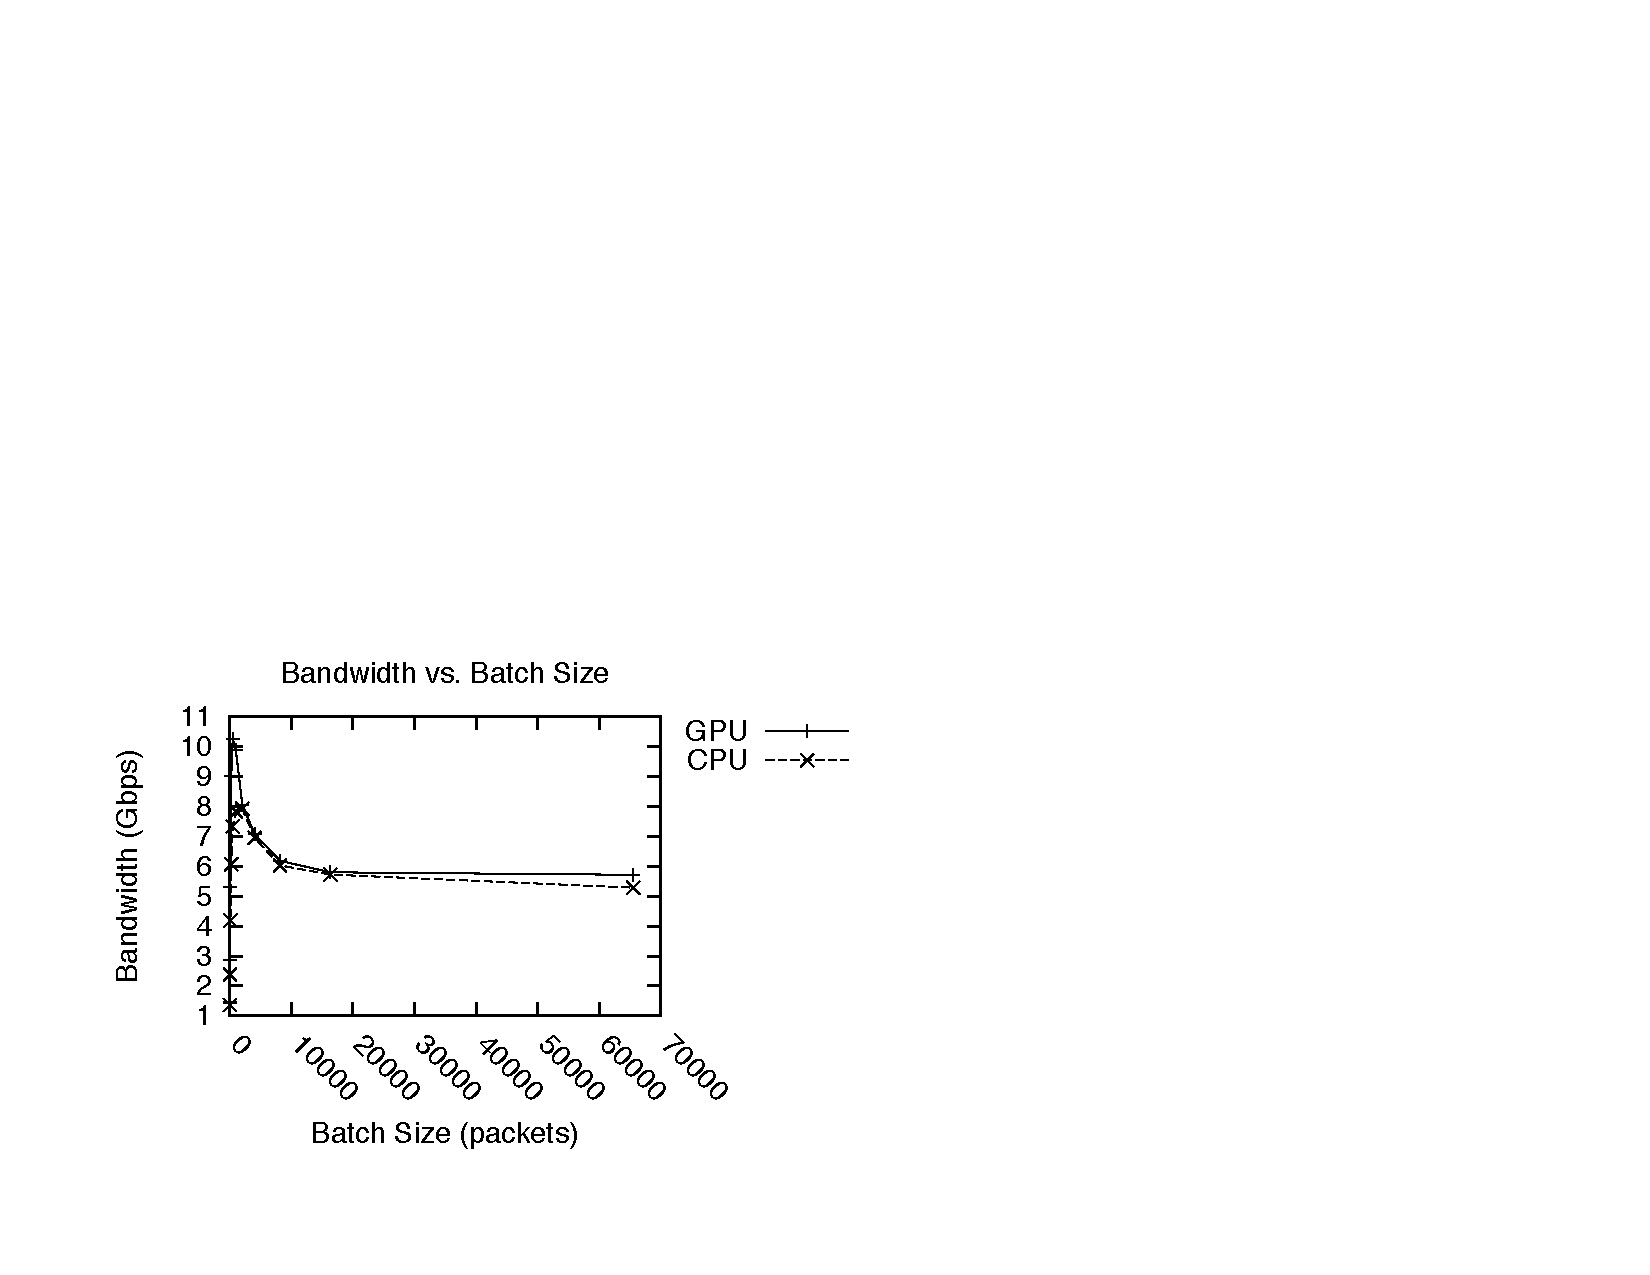
\includegraphics[height=4cm]{figs/batch_size_header_pinned_both_par_bw.pdf}\label{fig:iter3-bw}}

	\medskip
    \subfigure[Latency vs. Batch Size]{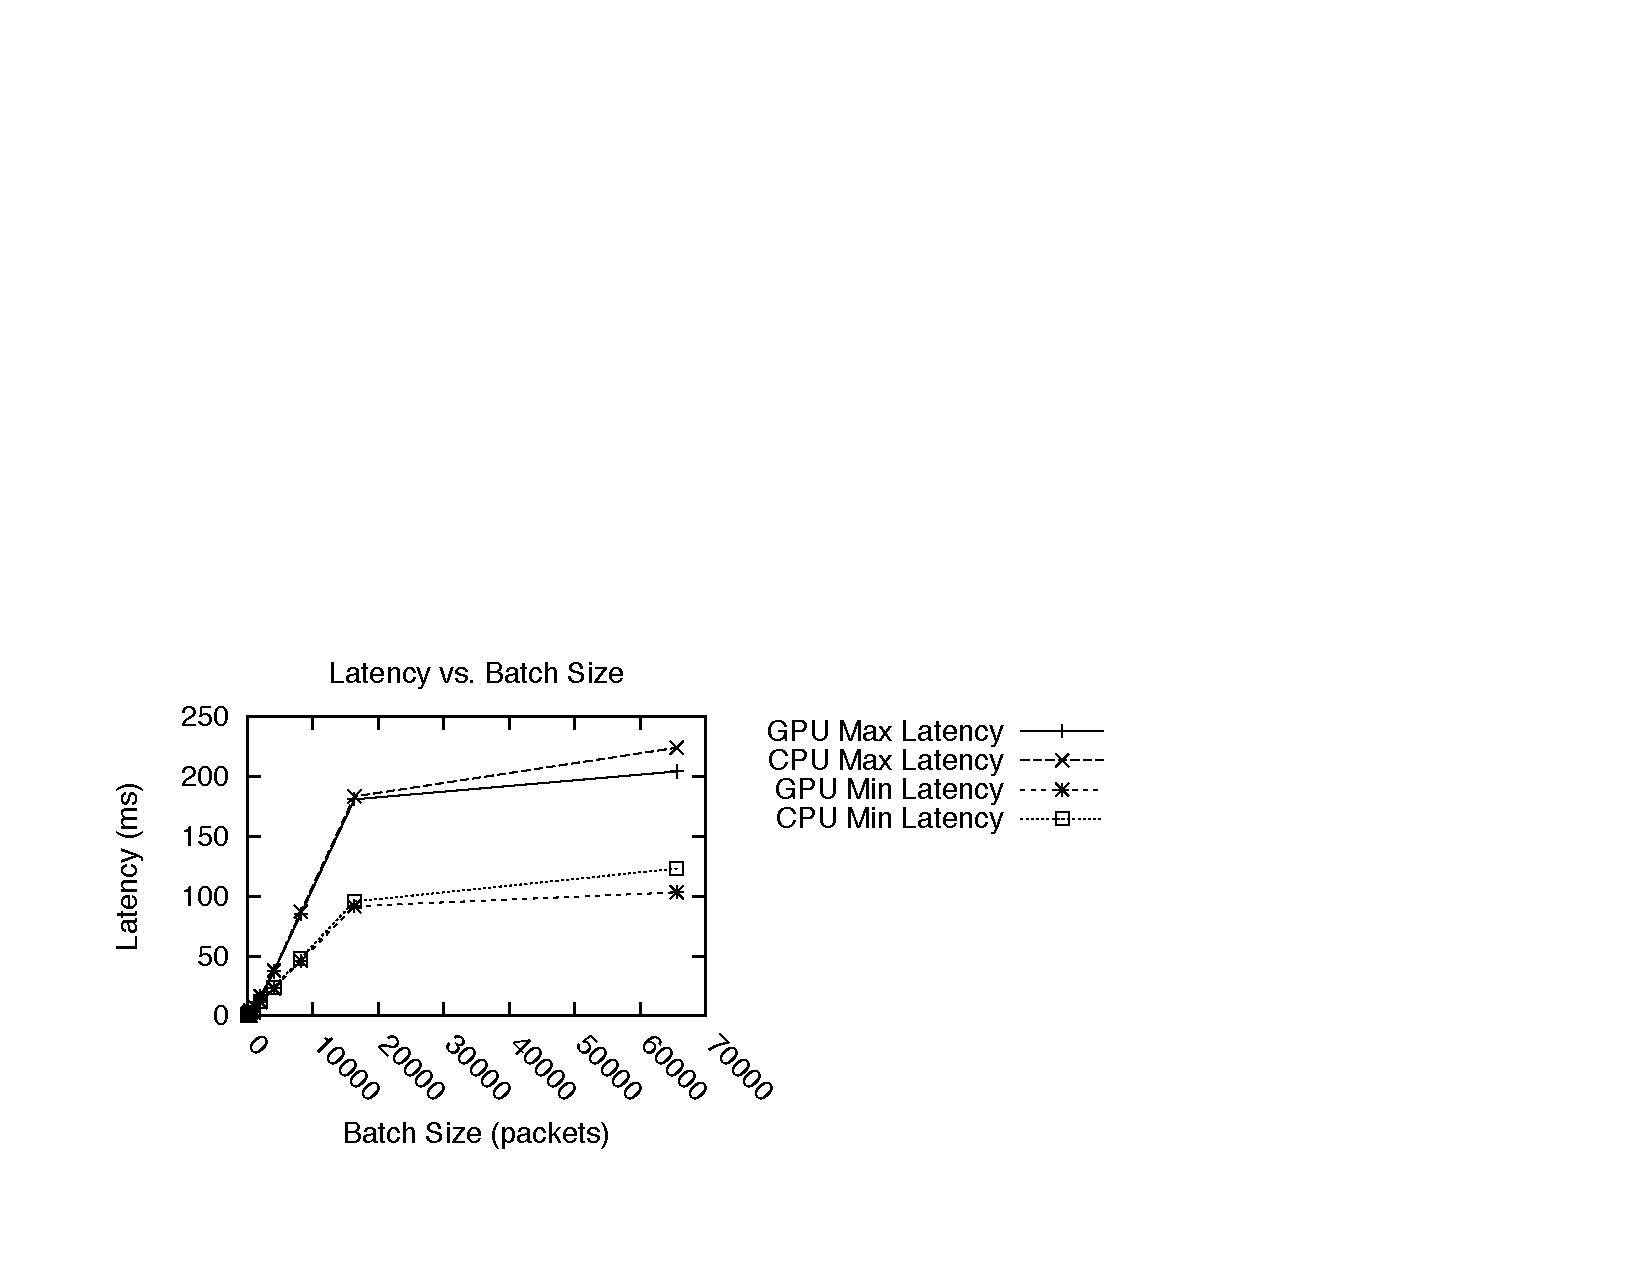
\includegraphics[height=4cm]{figs/batch_size_header_pinned_both_par_lat.pdf}\label{fig:iter3-lat}}

   	\medskip
	\subfigure[Breakdown of GPU Time]{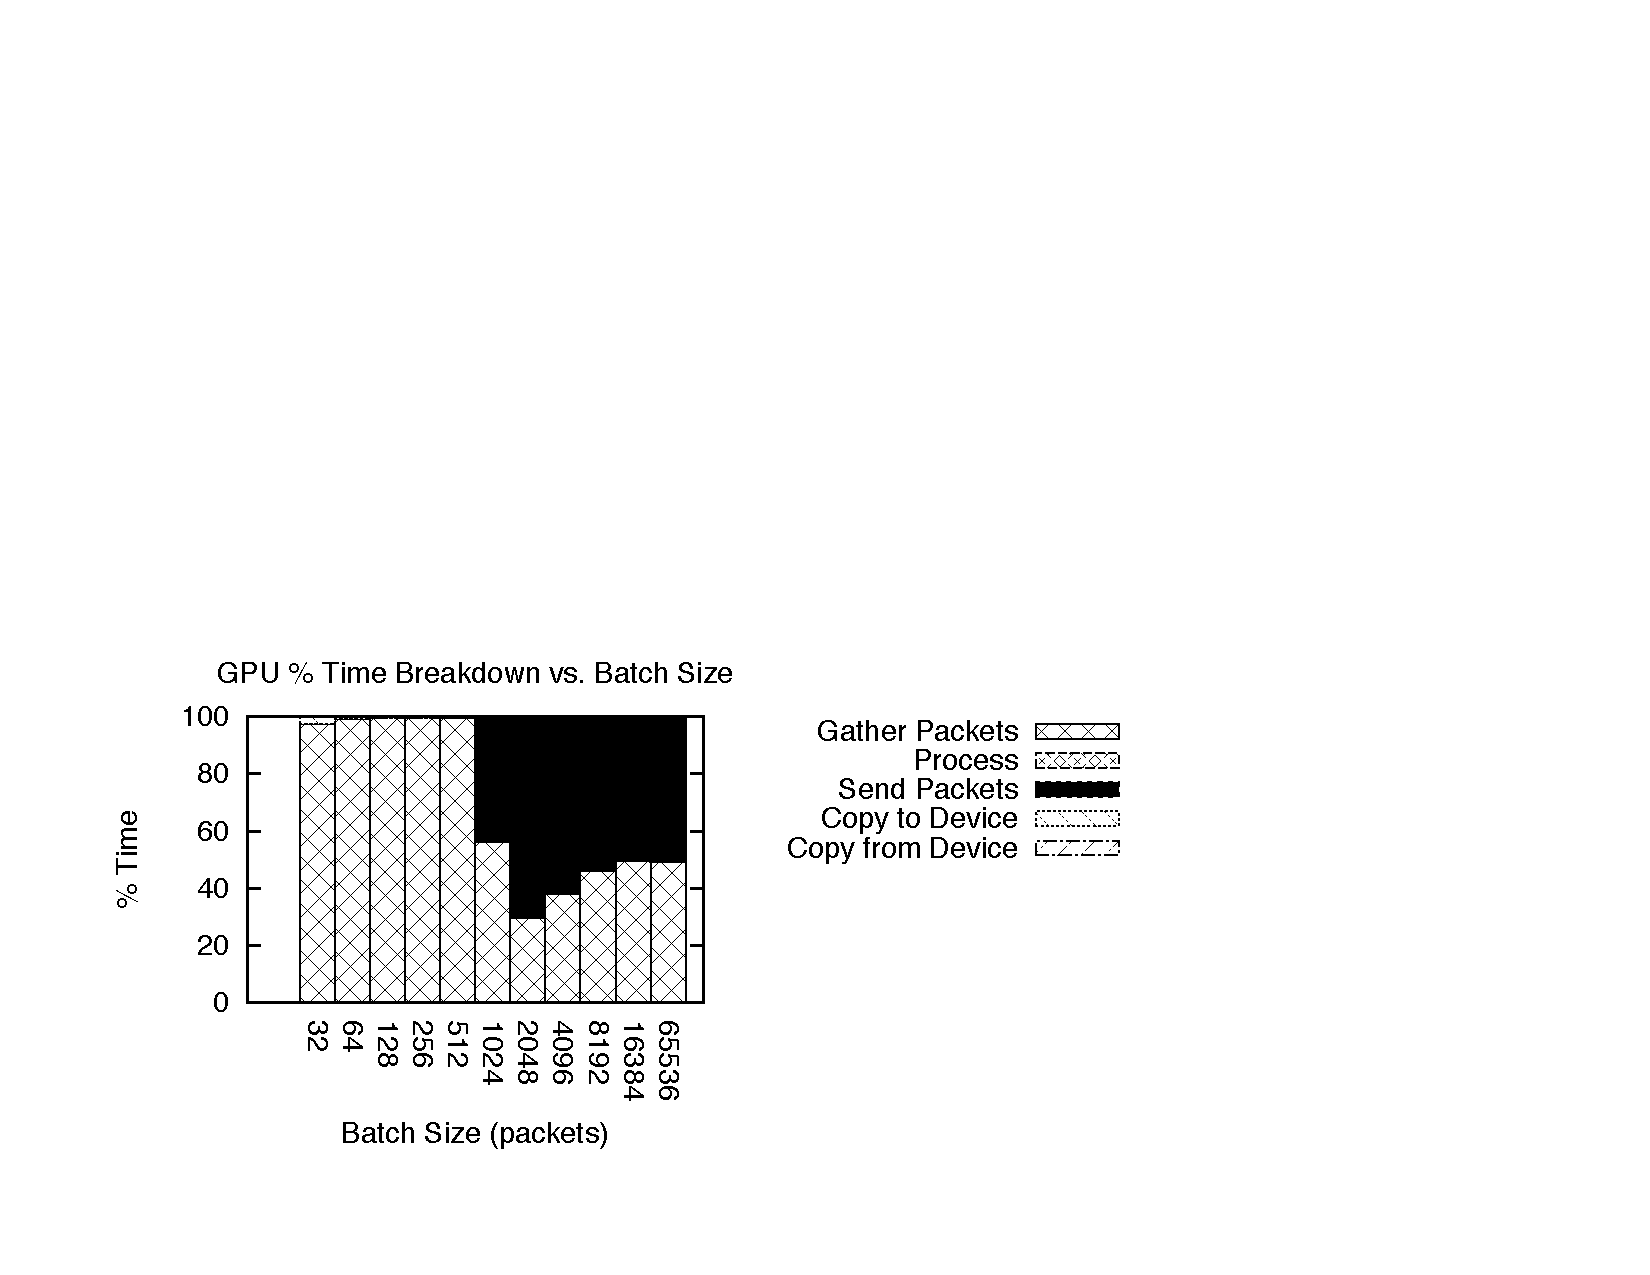
\includegraphics[height=4cm]{figs/batch_size_header_pinned_both_par_gpu_p.pdf}\label{fig:iter3-gpu-breakdown}}

    \caption{Iteration 3 Results}
	\label{fig:iter3}
\end{figure}


\subsubsection{Iteration Four}

\TODO{Talk about eliminating gather / send time, and how this at least indicates that with better IO we would do very well.}


\begin{figure*}
    \centering
    \subfigure[Bandwidth vs. Batch Size]{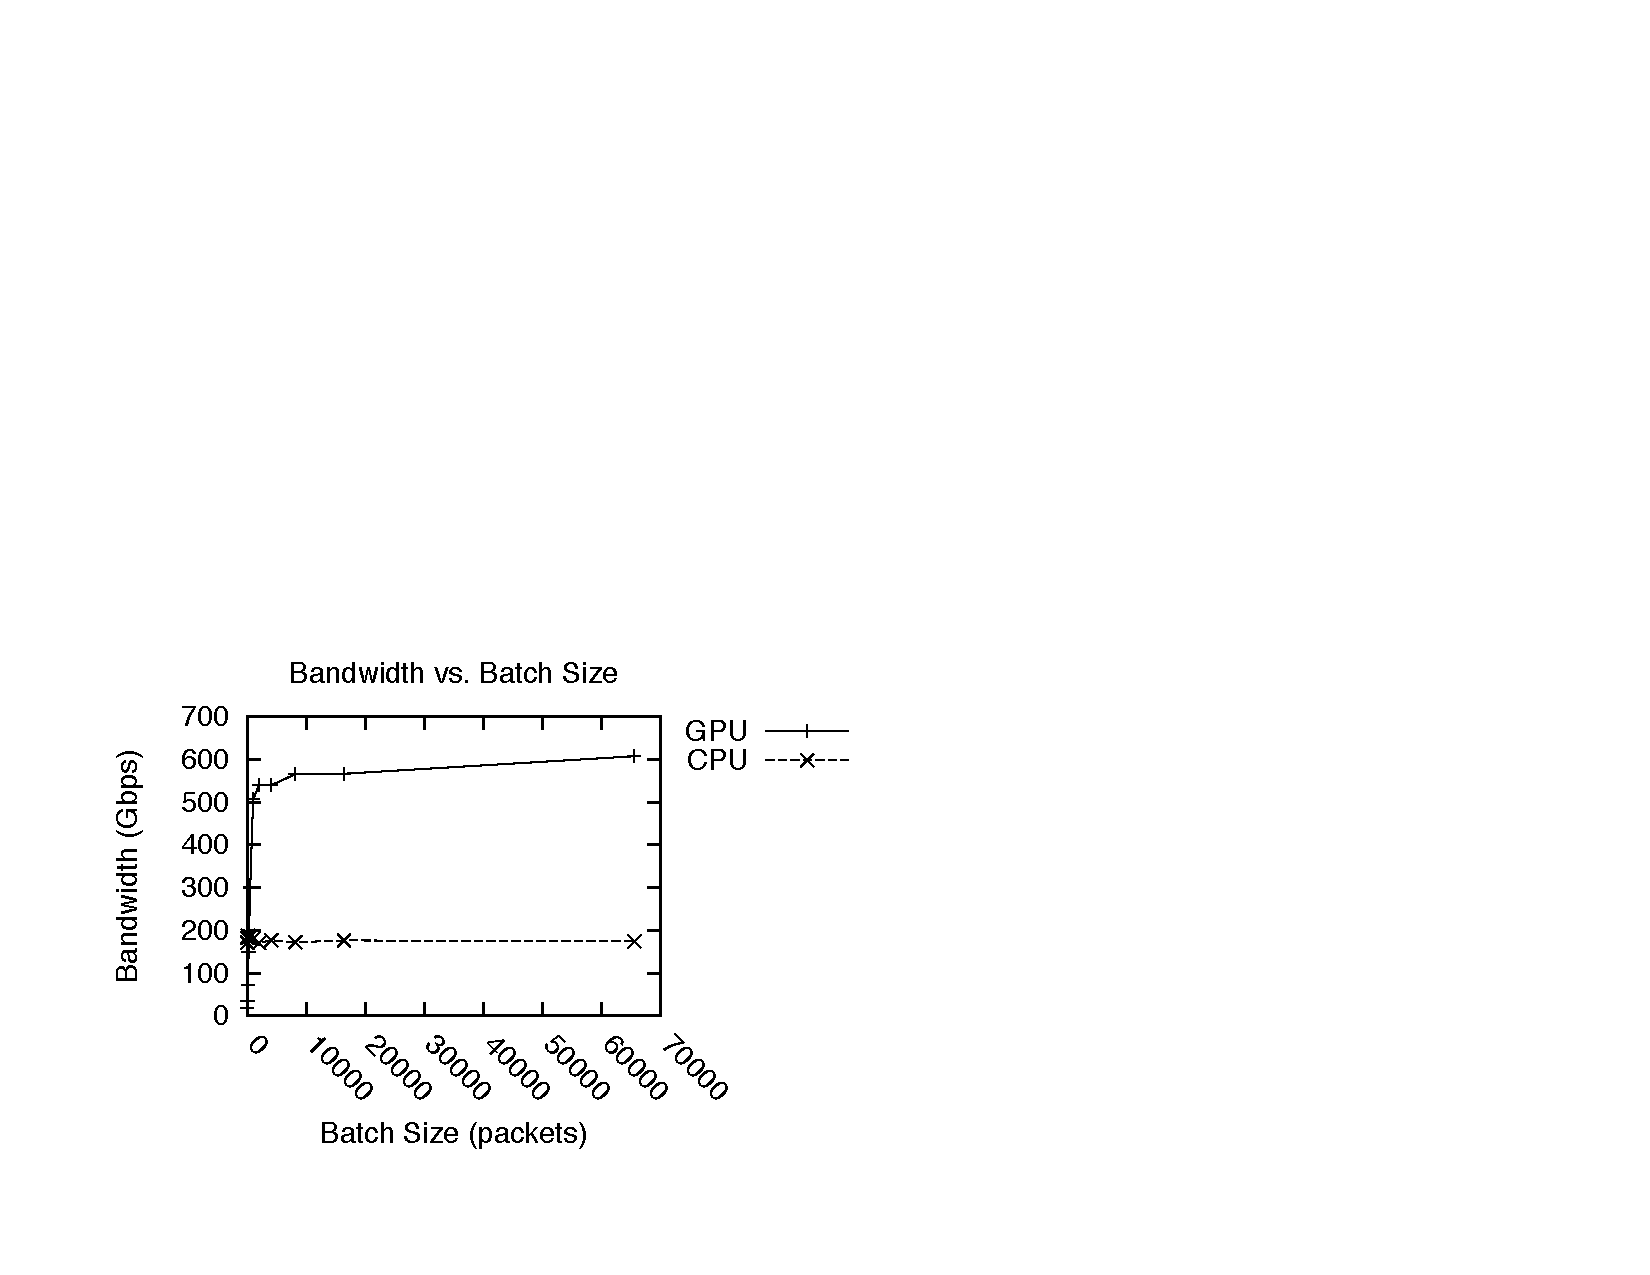
\includegraphics[height=4.5cm]{figs/batch_size_header_pinned_immediate_both_par_bw.pdf}\label{fig:iter4.5-bw}}
	\quad
    \subfigure[Latency vs. Batch Size]{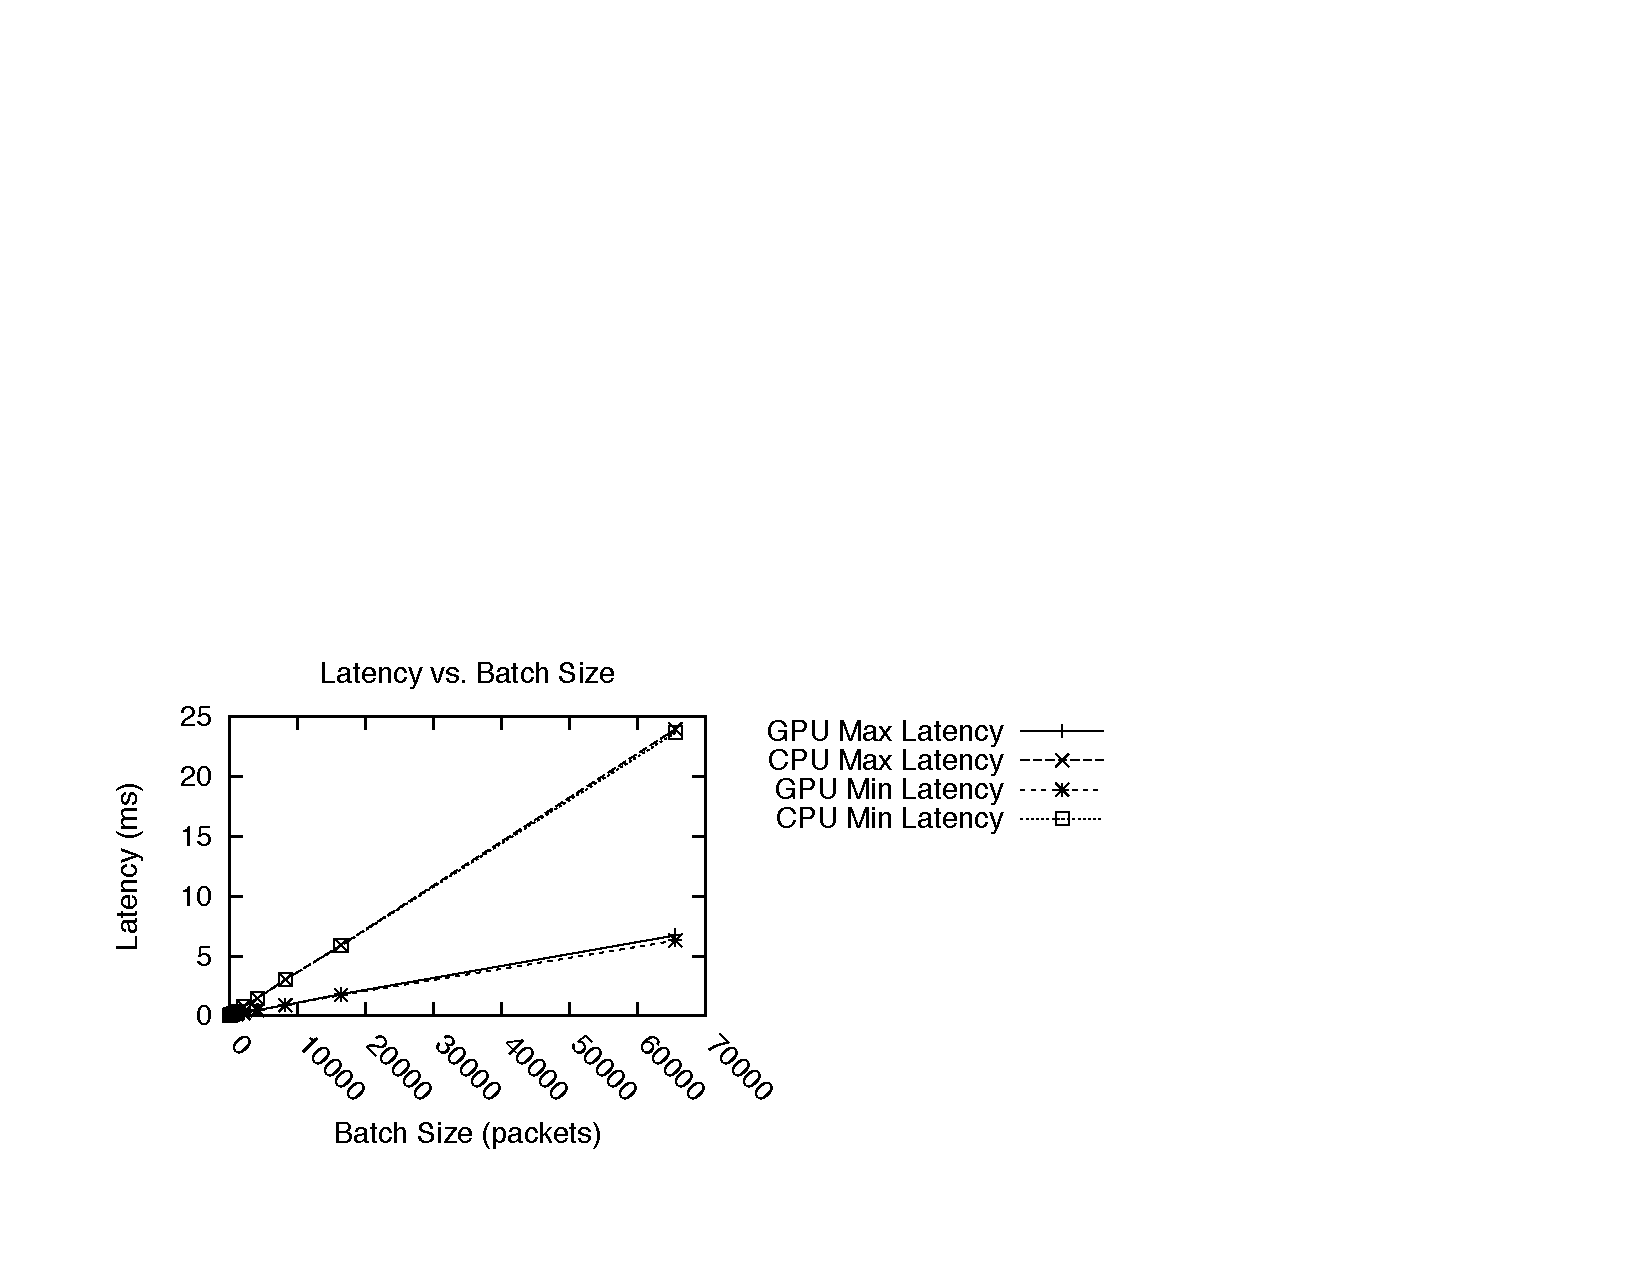
\includegraphics[height=4.5cm]{figs/batch_size_header_pinned_immediate_both_par_lat.pdf}\label{fig:iter4.5-lat}}

    \caption{Iteration 4 Results}
	\label{fig:iter4}
\end{figure*}
